\begin{figure}[H]
  \centering
  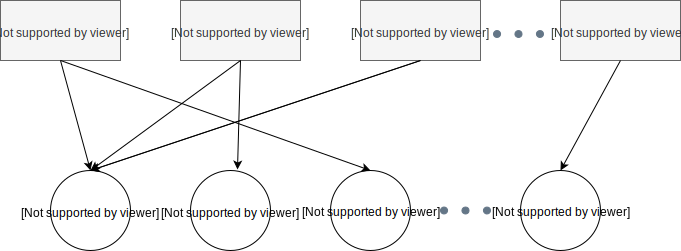
\includegraphics[width=80mm, height=30mm]{figures/dag.png}
  \caption{Graph representation of a parameter sweep application.}
  \label{fig:dag}
\end{figure}

\section{background} \label{sec:background}

\subsection*{Parameter Sweep Applications}

Scientific applications are often represented as directed acyclic graphs (DAGs)
where nodes represent computational tasks and input/output files. Links
generally will start at a file and extend to a task or vice versa. A link from a
file to a task denotes that the task requires the file as an input. Conversely,
a link from a task to a file signifies that the task creates that file as its
output. Here we focus on one such scientific application known as a parameter
sweep, where there are an independent set of $n$ files $f_j$, $1 \leq j \leq n$ and $m$ tasks $t_k$, $1 \leq k \leq m$ as depicted in Figure~\ref{fig:dag}.
These files have links to tasks, thus forming a bipartite graph. Depending on the
application, this bipartite graph may be arranged in a number of ways. For
example, consider an application with 10 files and 20 tasks. And say, each file
is used by a pair of tasks. This type of application may be easily parallelized
as the graph can be partitioned into sections. However, in the case of irregular
applications, the dependencies between files and tasks can make it difficult to
effectively schedule it onto a set of hardware resources. Scheduling the
execution on a single compute resource is trivial, but beyond that, the
scheduling problem is shown to be NP-Complete in many cases
\cite{Giersch-task-sharing-files-04}. Even when executed on modern day,
massively parallel compute architectures, these scientific applications can be
so large that they take days or months to execute.

\begin{figure}[H]
  \centering
  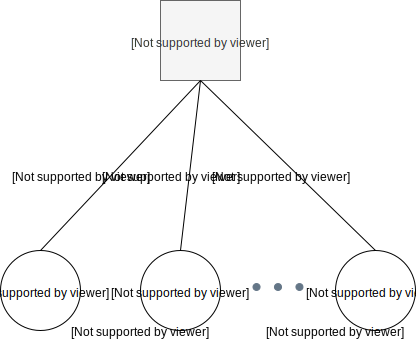
\includegraphics[width=50mm, height=40mm]{figures/platform.png}
  \caption{Master worker infrastructure.}
  \label{fig:platform}
\end{figure}

\subsection*{Cyberinfrastructure}

The focus of this project is scheduling a parameter sweep application onto a
cyberinfrastructure arranged in a \textit{master worker} layout shown in Figure~\ref{fig:platform}. The
master node is connected to $k$ worker nodes, $w_i$ where $1 \leq i \leq k$.
The links between master and worker nodes, $l_i$ where $1 \leq i \leq k$ have
a bandwidth of $bw_i$, denoted in megabytes per second (MBps).
Worker node $w_i$ has a compute speed $c_i$ denoted in floating point operations
per second (flops).

The master is responsible for assigning tasks to workers. Depending
on the application graph, before the master can map a task to a worker,
that tasks's required input files must be present at a persistant storage
service located on that same worker. Here we restrict the master from
sending more than one file at a time to a worker. Additionally the master
may start up a task at any moment on a worker if the required files are present
at the worker's persistant storage. Once a file has been sent from the master
to some worker, that file will be retained by the worker and may be used by
multiple tasks. Furthermore, the master may send the same file to multiple
workers such that multiple tasks that require the same file may be executed
in parallel by different workers.

Consider a simple application comprised of a single task $t$ that requires
some number of floating point operations to complete. $t$ also requires the set
of $F$ files. The master will synchronously send each file in $F$ to $w_1$
over $l_1$ then instruct $w_1$ to execute $t$. The expected makespan of this
particular application can be modeled by the following equation:
$$ makespan_{expected} = \frac{\sum\limits_{f \in F}size(f)}{bw_1} + \frac{num\_flops(t)} {c_1} $$
Modeling expected execution times is used by a number of scheduling heuristics
including Max-Min and Min-Min.

\subsection*{List Scheduling Heuristics}

Two of the most common online list scheduling algorithms are Max-Min and Min-Min.
Both of these algorithms use estimated minimum completion times (MCT) of each
task to determine which set of files and tasks to map to what resource by
computing the following:

\begin{algorithm}[H]
  \renewcommand{\thealgorithm}{}
  \caption{Estimate MCT}
  \begin{algorithmic}
    \STATE $ECTS = [|pending\_tasks|][|workers|]$
    \FOR{$t \in pending\_tasks$}
      \FOR{$w \in workers$}
        \STATE $ect = estimate\_completion\_time(t, w)$
        \STATE $ECTS[t][w] = ect$
      \ENDFOR
    \ENDFOR
  \end{algorithmic}
\end{algorithm}

\subsubsection*{Max-Min}
first selects the task with the maximum of all the minimum estimated completion time.
Then, that task is assigned to the worker which will give it the largest estimated
completion
time out of all the possible workers it could have run on. This is to start long
tasks early on slower resources such that smaller tasks can be executed faster
on fast resources.

\subsubsection*{Min-Min}
selects the task, worker pair with the fastest estimated completion time and
assigns that task to that worker.
